\section{How to Use}
After starting the application, click an option from the tool-bar.
If you've clicked on an action, you can draw to the canvas by clicking once to start and a second time to complete the shape.
\begin{center}\fbox{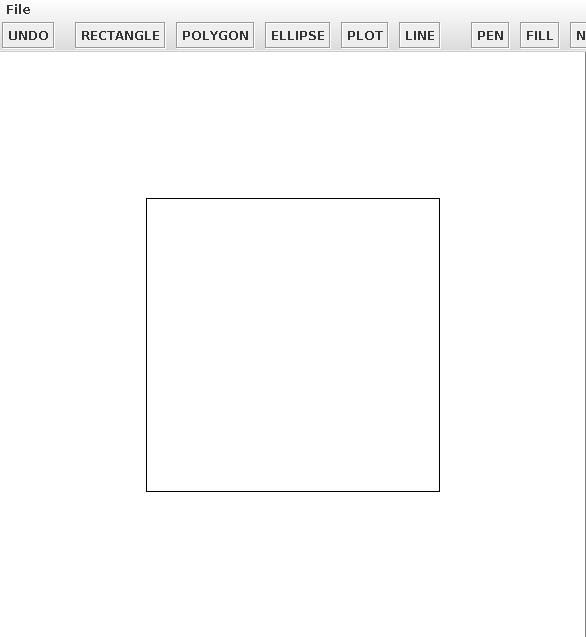
\includegraphics[width=0.6\textwidth]{./images/main.png}}\end{center}
If you've selected the polygon option, left-click to add a point and then right-click to add the final point and complete the polygon.
To select a fill or pen colour, click the pen or fill option.
\begin{center}\fbox{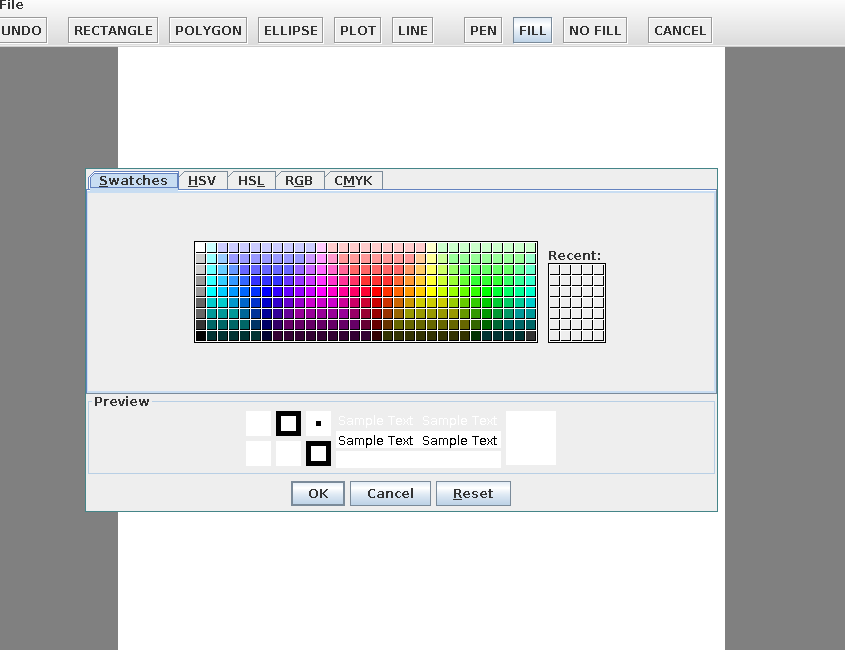
\includegraphics[width=0.6\textwidth]{./images/color-picker.png}}\end{center}
A dialog with a palette will open up, selecting a colour will apply to actions that follow.
\begin{center}\fbox{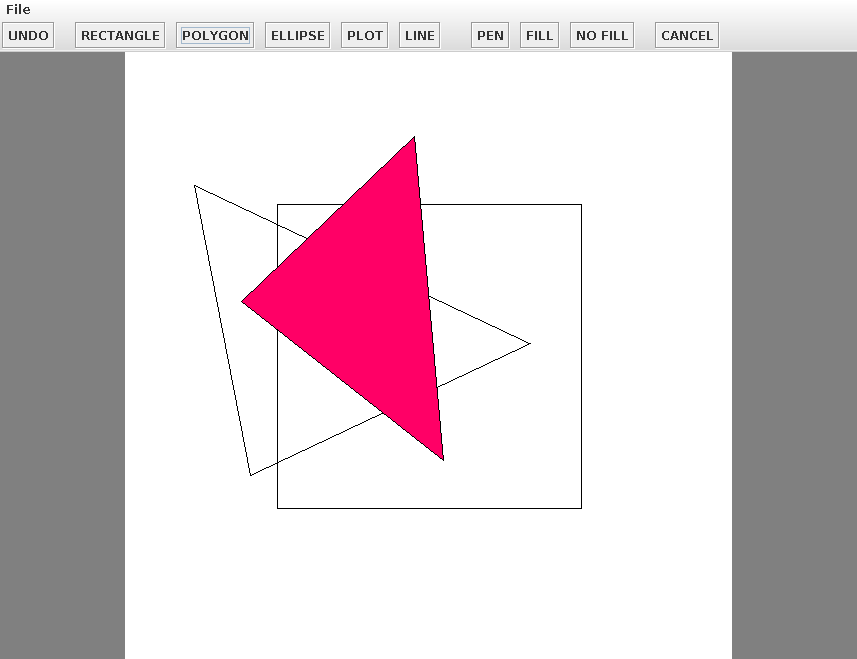
\includegraphics[width=0.6\textwidth]{./images/colored.png}}\end{center}
Finally, to save the new vector select Save from the File menu.
